\documentclass[14pt,a4paper,report]{report}
\usepackage[a4paper, mag=1000, left=2.5cm, right=1cm, top=2cm, bottom=2cm, headsep=0.7cm, footskip=1cm]{geometry}
\usepackage[utf8]{inputenc}
\usepackage[english,russian]{babel}
\usepackage{indentfirst}
\usepackage[dvipsnames]{xcolor}
\usepackage[colorlinks]{hyperref}
\usepackage{listings} 
\usepackage{fancyhdr}
\usepackage{caption}
\usepackage{amsmath}
\usepackage{graphicx}
\usepackage{amsmath}
\usepackage{booktabs}
\usepackage{array}
\newcolumntype{P}[1]{>{\centering\arraybackslash}p{#1}}
\hypersetup{
colorlinks = true,
linkcolor = black
}

\usepackage{titlesec}
\titleformat{\chapter}
{\Large\bfseries} % format
{} % label
{0pt} % sep
{\huge} % before-code


\DeclareCaptionFont{white}{\color{white}} 

% Listing description
\usepackage{listings} 
\DeclareCaptionFormat{listing}{\colorbox{gray}{\parbox{\textwidth}{#1#2#3}}}


\captionsetup[lstlisting]{format=listing,labelfont=white,textfont=white}
\lstset{ 
% Listing settings
inputencoding = utf8,	
extendedchars = \true, 
keepspaces = true, % Поддержка кириллицы и пробелов в комментариях
language = C, % Язык программирования (для подсветки)
basicstyle = \small\sffamily, % Размер и начертание шрифта для подсветки кода
keywordstyle=\color{blue}\ttfamily,
stringstyle=\color{red}\ttfamily,
commentstyle=\color{green}\ttfamily,
morecomment=[l][\color{magenta}]{\#},
numbers = left, % Где поставить нумерацию строк (слева\справа)
numberstyle = \tiny, % Размер шрифта для номеров строк
stepnumber = 1, % Размер шага между двумя номерами строк
numbersep = 5pt, % Как далеко отстоят номера строк от подсвечиваемого кода
backgroundcolor = \color{white}, % Цвет фона подсветки - используем \usepackage{color}
showspaces = false, % Показывать или нет пробелы специальными отступами
showstringspaces = false, % Показывать или нет пробелы в строках
showtabs = false, % Показывать или нет табуляцию в строках
frame = single, % Рисовать рамку вокруг кода
tabsize = 2, % Размер табуляции по умолчанию равен 2 пробелам
captionpos = t, % Позиция заголовка вверху [t] или внизу [b] 
breaklines = true, % Автоматически переносить строки (да\нет)
breakatwhitespace = false, % Переносить строки только если есть пробел
escapeinside = {\%*}{*)} % Если нужно добавить комментарии в коде
}

\begin{document}

\def\contentsname{Содержание}

% Titlepage
\begin{titlepage}
\begin{center}
\textsc{Санкт-Петербургский Политехнический 
Университет Петра Великого\\[5mm]
Кафедра компьютерных систем и программных технологий}

\vfill

\textbf{Отчёт по лабораторной работе №3-4\\[3mm]
на тему: «Визуализация каркасной модели»\\[3mm]
Курс: «Разработка графических приложений»\\[41mm]
}
\end{center}

\hfill
\begin{minipage}{.4\textwidth}
Выполнил студент:\\[2mm] 
Волкова М.Д.\\
Группа: 13541/2\\[5mm]

Проверил:\\[2mm] 
Абрамов Н.А.
\end{minipage}
\vfill
\begin{center}
Санкт-Петербург\\ \the\year\ г.
\end{center}
\end{titlepage}

% Contents
\tableofcontents
\clearpage

\chapter{Лабораторная работа №2}

\section{Цель работы}
Разработать программу на языке С для растеризации загруженной модели на экран

\section{Описание программы}
\begin{enumerate}
\item Возможности программы:
\begin{enumerate}
\item Загрузка трехмерной модели из OBJ-файла
\item Растеризация каркаса трехмерной модели
\item Обеспечение вращения камеры вокруг трехмерной модели
\item Растеризация линий своим алгоритмом
\item Растеризация треугольников своим алгоритмом
\item Вычисление координат и получение значения глубины для конкретного пикселя
\item Использования буффера глубины для отсечения невидимых пикселей
\end{enumerate}
\item Входные параметры программы:
\begin{enumerate}
\item Ширина и высота окна
\item Вертикальный угол обзора камеры для выполненя перспективной проекции
\item Ближняя и дальняя плоскости отсечения камеры
\item Дистанция от камеры до загруженной модели
\item Скорость вращения камеры вокруг модели (градус/сек)
\end{enumerate}
\item Выходные параметры программы:
\begin{enumerate}
\item Последовательность кадров, выводимая на экран
\end{enumerate}
\item Порядок работы программы:
\begin{enumerate}
\item Загрузка трехмерной модели в вершинные и индексные буфера
\item Определение центра модели (можно считать, что матрица мира для модели – единичная)
\item Формирование матрицы проекции
\item Далее – для очередного кадра:
\begin{enumerate}
\item Формирование матрицы вида исходя из координат центра модели, дистанции до модели и скорости вращения камеры
\item Преобразование вершин модели в экранные координаты 
\end{enumerate}
\end{enumerate}
\end{enumerate}
\clearpage

\section{Ход работы}
В дополнение к уже установленной ранее библиотеке OpenCV дополнительно была установлена библиотека GLM, предназначенная для работы с векторами и матрицами размерности до 4-х. Для работы с форматом OBJ использована библиотека TinyObj.

Программа предоставлена в листинге.
\subsection{Алгоритм Брезенхема}

Алгоритм Брезенхема - это алгоритм, определяющий, какие точки двумерного растра нужно закрасить, чтобы получить близкое приближение прямой линии между двумя заданными точками.

Для проволочного рендеринга, сначала нам нужна функция, оторая будет отрисовывать линии:
\begin{lstlisting}
    template<typename F>
    inline void drawline(int x0, int y0, int x1, int y1, F plot) {

        int dx = std::abs(x1 - x0);
        int dy = std::abs(y1 - y0);

        int directionX = x0 < x1 ? 1 : -1;
        int directionY = y0 < y1 ? 1 : -1;
        int err = (dx > dy ? dx : -dy) / 2;

        for (;;) {
            plot(x0, y0);
            if (x0 == x1 && y0 == y1) break;
            int e2 = err;
            if (e2 > -dx) {
                err -= dy;
                x0 += directionX;
            }
            if (e2 < dy) {
                err += dx;
                y0 += directionY;
            }
        }
    }
\end{lstlisting}


Для хранения модели мы используем формат wavefront obj. Формат файлов OBJ - это простой формат данных, который содержит только 3D геометрию, а именно, позицию каждой вершины, связь координат текстуры с вершиной, нормаль для каждой вершины, а также параметры, которые создают полигоны.Всё, что нам нужно для рендера, это прочитать из файла массив вершин вида:

\begin{lstlisting}
 v 0.608654 -0.568839 -0.416318 
\end{lstlisting}
это координаты x,y,z, одна вершина на строку файла и граней:
\begin{lstlisting}
f 7 6 1 
\end{lstlisting}
еще в файле содержиться нормали (нормали могут быть не нормированными):
\begin{lstlisting}
vn -0.966742 -0.255752 9.97231e-09 
\end{lstlisting}
Нас интересуют первое число после каждого пробела, это номер вершины в массиве, который мы прочитали ранее. Таким образом эта строчка говорит, что вершины 7, 6 и 1 образуют треугольник.

Далее пишем функцию, которая принимает объект класса Drawer, вершины и координаты модели и рисует линии:
\begin{lstlisting}
void render(Drawer &drawer, const std::vector<glm::vec3> &vertices, const std::vector<unsigned int> &indices) {
    for (auto i = 0; i < indices.size(); i += 3) {
        Triangle triangle{vertices[indices[i]], vertices[indices[i + 1]], vertices[indices[i + 2]]};
        drawer.draw(triangle);
    }
}
\end{lstlisting}

\subsection{Настройка фиксированной камеры}
В OpenGL при использовании фиксированного конвейера есть ровно две матрицы, относящихся к трансформациям точек и объектов:
\begin{itemize}

\item GL PROJECTION моделирует ортографическое или перспективное преобразование от трёхмерной усечённой пирамиды (т.е. от области видимости камеры) к трёхмерному кубу с длиной ребра, равной 2 (т.е. к нормализованному пространству).
\item GL MODELVIEW сочетает в себе два преобразования: от локальных координат объекта к мировым координатам, а также от мировых координат к координатам камеры.
\end{itemize}

За рамками фиксированного конвейера можно использовать столько матриц, сколько захочется. 

\begin{itemize}
\item поведение камеры описывается как ортографическим или перспективным преобразованием, так и положением камеры в мировом пространстве, то есть для моделирования камеры нужны GL PROJECTION и GL MODELVIEW одновременно
\item c другой стороны, для трансформаций над телами —  вращение предмета с помощью умножения координат на матрицу — нужна матрица GL MODELVIEW.
\end{itemize}

Настроим матрицу GL PROJECTION один раз для перспективного преобразования, а матрицу GL MODELVIEW будем постоянно модифицировать, когда локальная система координат очередного объекта не совпадает с мировой системой координат.

Начнём настройку камеры с GL MODELVIEW: зададим матрицу так, как будто бы камера смотрит с позиции camera position на точку model center, при этом направление “вверх” камеры задаёт вектор glm::vec3(0, 1, 0):

\begin{lstlisting}
camera = glm::lookAt(
                camera_position,
                model_center,
                glm::vec3(0, 1, 0)
        );
\end{lstlisting}
, где:
\begin{itemize}
\item camera position - Позиция камеры в мировом пространстве

\item model center - Указывает куда вы смотрите в мировом пространстве

\item glm::vec3(0, 1, 0) - Вектор, указывающий направление вверх

\end{itemize}

А вот диаграмма, которая показывает то, что мы делаем:
\begin{figure}[h!]
\center{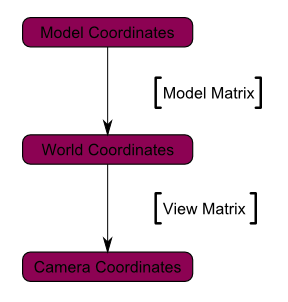
\includegraphics[width=0.35\linewidth]{images/diag.png}}
\label{ris:image}
\end{figure}

Для перспективного преобразования достаточно создать матрицу с помощью функции glm::perspective. Она принимает на вход несколько  параметров преобразования: горизонтальный угол обзора камеры, соотношение ширины и высоты, а также две граничных координаты для отсечения слишком близких к камере и слишком далёких от камеры объектов. 

Эти параметры легко увидеть на следующей иллюстрации:

\begin{figure}[h!]
\center{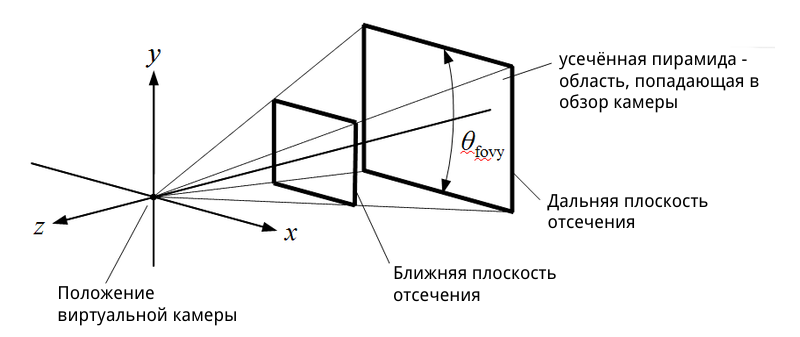
\includegraphics[width=0.8\linewidth]{images/perspective_volume.png}}
\label{ris:image}
\end{figure}

\subsubsection{Проекционная матрица}

Теперь мы находимся в пространстве камеры, вершина, которая получит координаты x == 0 и y == 0 будет отображаться по центру экрана. Однако, при отображении объекта огромную роль играет также дистанция до камеры. Для двух вершин, с одинаковыми x и y, вершина имеющая большее значение по z будет отображаться ближе, чем другая.

Это называется перспективной проекцией, к счастью, в glm имеем:
\begin{lstlisting}
projection = glm::perspective(
            glm::radians(fovy),
            screen_ratio,
            front,
            back)
\end{lstlisting}
, где:
\begin{itemize}
\item glm::radians(fovy) - Вертикальное поле зрения в радианах.

\item screen ratio - Отношение сторон.

\item front - Ближняя плоскость отсечения.

\item back - Дальняя плоскость отсечения.

\end{itemize}

Теперь наша диаграмма будет выглядеть так:
\begin{figure}[h!]
\center{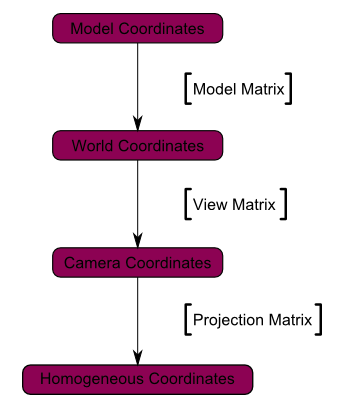
\includegraphics[width=0.45\linewidth]{images/diag2.png}}
\label{ris:image}
\end{figure}

\subsubsection{Матрица поворота}
Функция rotate в glm поворачивает 3D вектор на заданный угол вокруг заданной оси (представленной орт-вектором):
\begin{lstlisting}
glm::rotate(glm::mat4(1), angle, glm::vec3(0, 1, 0));
\end{lstlisting}

Следующий шагом  объединяем трансформации, что реализуется по следующей формуле:
\begin{lstlisting}
camera_position = (rotation_matrix * start_camera_position)
\end{lstlisting}


\subsection{Z-буферизация}
Z-буферизация - это способ учёта удалённости элемента изображения. Представляет собой один из вариантов решения «проблемы видимости». Очень эффективен и практически не имеет недостатков, если реализуется аппаратно. 

Формальное описание алгоритма z-буфера таково:
\begin{enumerate}

\item Заполнить буфер кадра фоновым значением интенсивности или цвета.
\item  Заполнить z-буфер минимальным значением z.
\item  Преобразовать каждый многоугольник в растровую форму в произвольном порядке.
\item Для каждого Пиксел(x,y) в многоугольнике вычислить его глубину z(x,y).
\item Сравнить глубину z(х,у) со значением Zбуфер(х,у), хранящимся в z-буфере в этой же позиции.
\item Если z(х,у) > Zбуфер (х,у), то записать атрибут этого многоугольника (интенсивность, цвет и т. п.) в буфер кадра и заменить Zбуфер(х,у) на z(х,у). В противном случае никаких действий не производить.
\end{enumerate}


Поскольку у нас экран двумерный, то z-буфер тоже должен быть двумерным:
 \begin{lstlisting}
    cv::Mat1d zBufferDefaultValue(int height, int width) {
        return cv::Mat::ones(height, width, CV_64F) * 100000;
    }
 \end{lstlisting}
 
Затем в коде мы проходим по всем треугольникам и делаем вызов растеризатора, передавая ему и картинку, и z-буфер.

   \begin{lstlisting}
       void triangleBarycentric(const ExtendedTriangle &t, cv::Mat1d &zBuffer, const MipMap<8> &mipMap) {
        auto &&bbox = t.box();
        Coord from = bound(bbox.first);
        Coord to = bound(bbox.second);
        for (auto x = from.x; x <= to.x; ++x) {
            for (auto y = from.y; y <= to.y; ++y) {
                glm::dvec3 barycentric;
                bool pointInTriangle = get_barycentric(t, glm::vec4(x, y, 1, 1), barycentric);
                if (!pointInTriangle) continue;
                glm::dvec3 zInterpolated = glm::dvec3(t.a.z, t.b.z, t.c.z) * barycentric;
                double z = zInterpolated[0] + zInterpolated[1] + zInterpolated[2];
                if (z < zBuffer.at<double>(y, x)) {
                    zBuffer.at<double>(y, x) = z;

                    glm::dvec3 barycentricX, barycentricY;
                    get_barycentric(t, glm::vec4(x + 1, y, 1, 1), barycentricX);
                    get_barycentric(t, glm::vec4(x, y + 1, 1, 1), barycentricY);

                    glm::vec2 uv = interpolateTexture(t.texture, barycentric);
                    glm::vec2 uvX = interpolateTexture(t.texture, barycentricX);
                    glm::vec2 uvY = interpolateTexture(t.texture, barycentricY);

                    glm::vec2 dx = uvX - uv;
                    glm::vec2 dy = uvY - uv;

                    float l = std::max(glm::dot(dx, dx), glm::dot(dy, dy));
                    float d = std::max(0.0f, 0.5f * std::log2(l));

                    cv::Vec3b texel = trilinearFilter(uv, d, mipMap);
                    plot(x, y, texel);

                }
            }
        }
    }
    \end{lstlisting}

В этой функции мы переводим координаты в барицентрические, с помощью следующей функии:
\begin{lstlisting}
    bool get_barycentric(const ExtendedTriangle &t, const glm::vec4 &p, glm::dvec3 &barycentric) {
        auto area = edgeFunction(t.a, t.b, t.c);
        auto w0 = edgeFunction(t.b, t.c, p) / area;
        auto w1 = edgeFunction(t.c, t.a, p) / area;
        auto w2 = edgeFunction(t.a, t.b, p) / area;

        barycentric = glm::dvec3(w0, w1, w2);
        barycentric /= barycentric[0] + barycentric[1] + barycentric[2];
        barycentric = glm::abs(barycentric);

        return !(w0 < 0 || w1 < 0 || w2 < 0);
    }
    \end{lstlisting}
    
Все, что с отрицательным значением - отбрасываеться.

\begin{lstlisting}
        double min, max;
        cv::minMaxLoc(drawer.zBuffer, &min, &max);
        cv::Mat zNorm;
        cv::normalize(drawer.zBuffer, zNorm, 0.0, 255.0, cv::NORM_MINMAX, CV_8UC1);
       \end{lstlisting}

Функция minMaxLoc находит минимальное и максимальное значения элементов и их положения. 

normalize нормализует src таким образом, что минимальное значение выходного массива равно 0.0, а максимальное значение выходного массива равно 255.0. 





\clearpage
\section{Результаты}
В качестве тестовой модели для проверки работоспособности программы использовалась модель чайничка, экспортированная стандартными средствами в формат OBJ.

 


\subsection{CvLineDrawer}
Параметры:

\begin{figure}[h!]
\center{\includegraphics[width=1\linewidth]{images/CvLineDrawer/options.png}}
\caption{Параметры}
\label{ris:image}
\end{figure}

Результат работы: 

\begin{figure}[h!]
\begin{minipage}[h]{0.47\linewidth}
\center{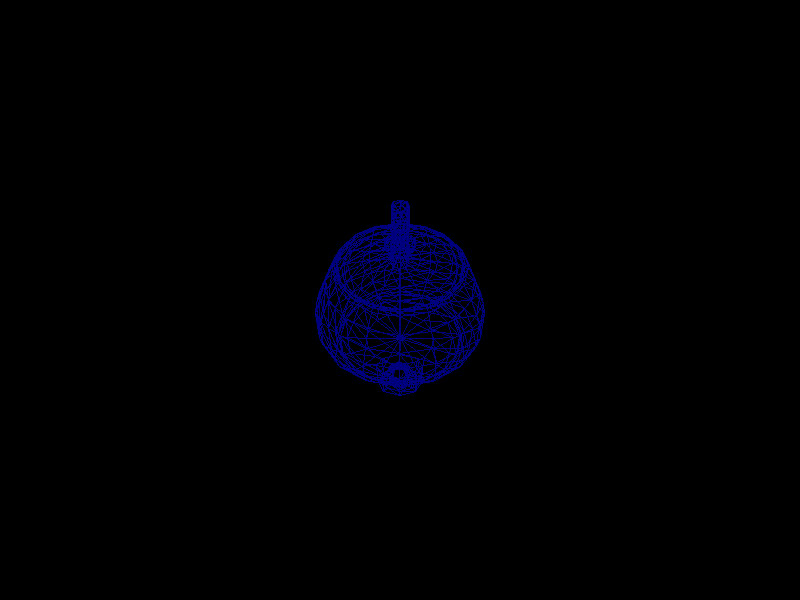
\includegraphics[width=1\linewidth]{images/CvLineDrawer/teapot0.png}} a) \\
\end{minipage}
\hfill
\begin{minipage}[h]{0.47\linewidth}
\center{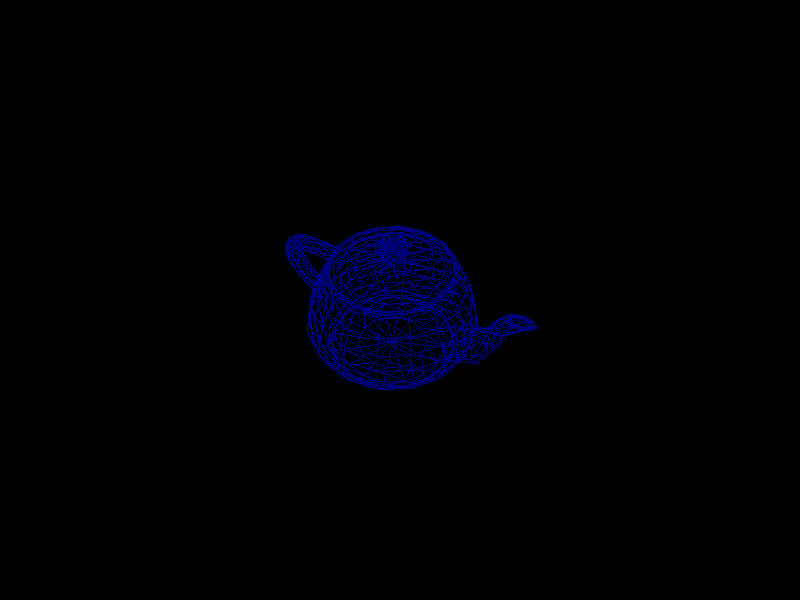
\includegraphics[width=1\linewidth]{images/CvLineDrawer/teapot1.png}} \\b)
\end{minipage}
\vfill
\begin{minipage}[h]{0.47\linewidth}
\center{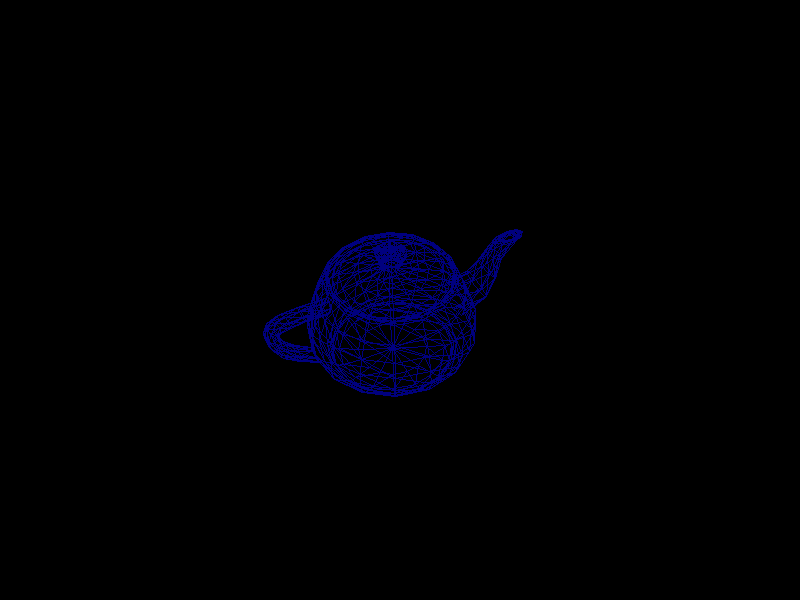
\includegraphics[width=1\linewidth]{images/CvLineDrawer/teapot2.png}} c) \\
\end{minipage}
\hfill
\begin{minipage}[h]{0.47\linewidth}
\center{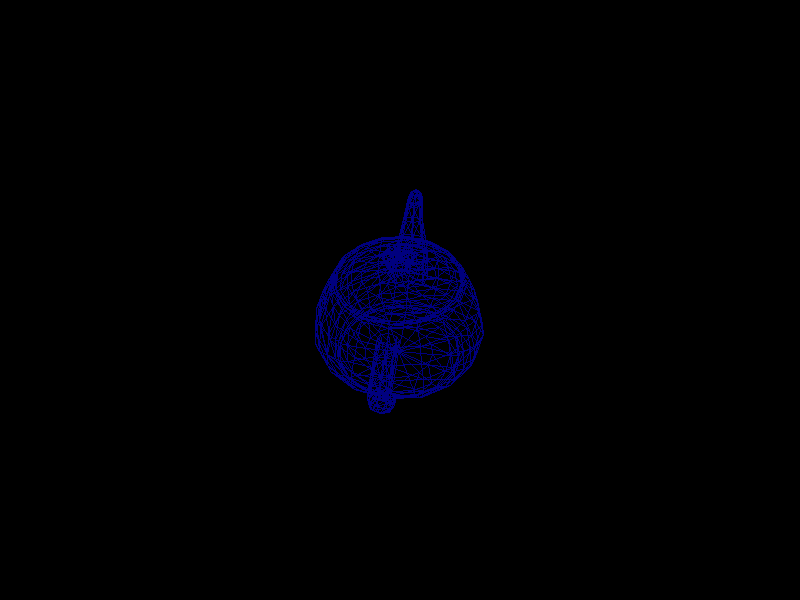
\includegraphics[width=1\linewidth]{images/CvLineDrawer/teapot3.png}} d) \\
\end{minipage}
\caption{Последовательно создаваемые изображения}
\label{ris:experimentalcorrelationsignals}
\end{figure}


\clearpage
\subsection{LineDrawer}
Параметры:

\begin{figure}[h!]
\center{\includegraphics[width=1\linewidth]{images/LineDrawer/options.png}}
\caption{Параметры}
\label{ris:image}
\end{figure}

Результат работы: 

\begin{figure}[h!]
\begin{minipage}[h]{0.47\linewidth}
\center{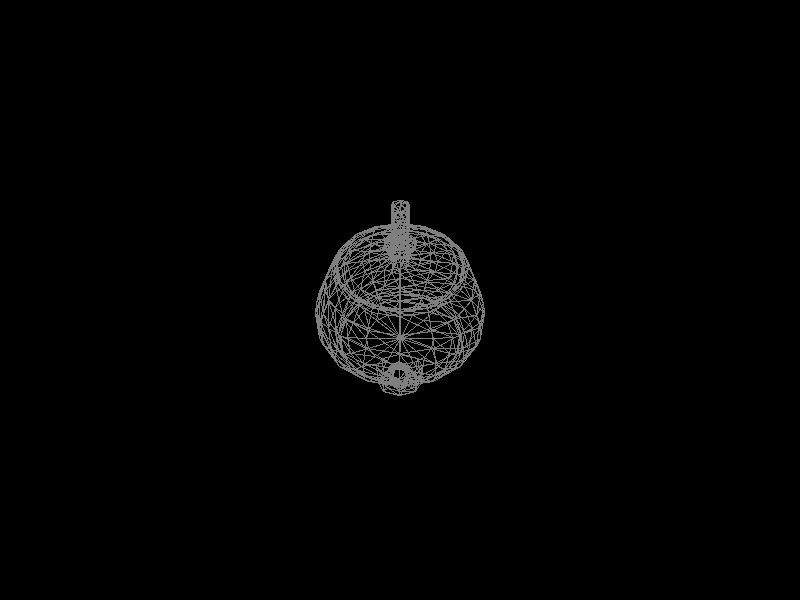
\includegraphics[width=1\linewidth]{images/LineDrawer/teapot0.png}} a) \\
\end{minipage}
\hfill
\begin{minipage}[h]{0.47\linewidth}
\center{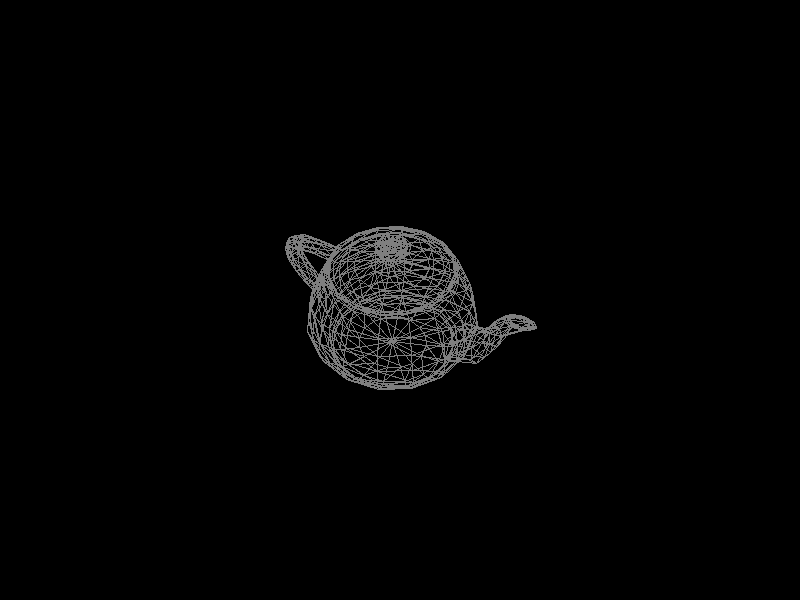
\includegraphics[width=1\linewidth]{images/LineDrawer/teapot1.png}} \\b)
\end{minipage}
\vfill
\begin{minipage}[h]{0.47\linewidth}
\center{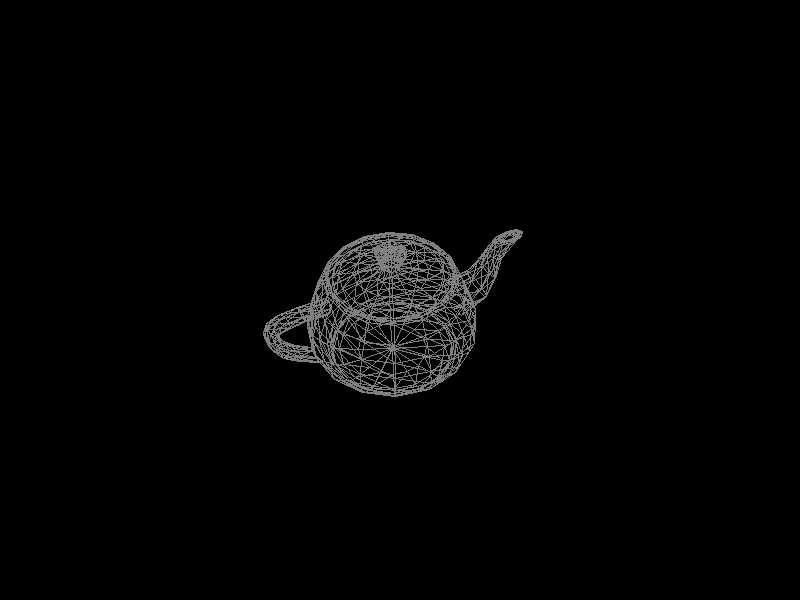
\includegraphics[width=1\linewidth]{images/LineDrawer/teapot2.png}} c) \\
\end{minipage}
\hfill
\begin{minipage}[h]{0.47\linewidth}
\center{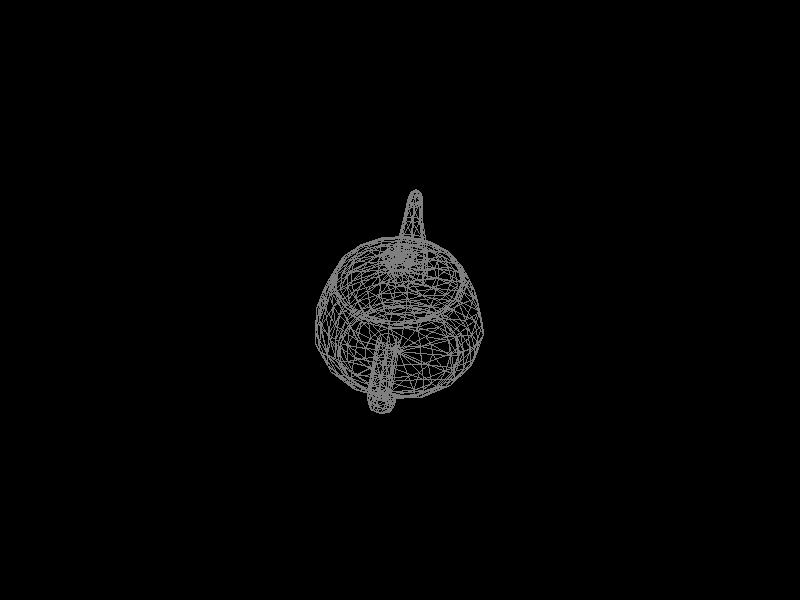
\includegraphics[width=1\linewidth]{images/LineDrawer/teapot3.png}} d) \\
\end{minipage}
\caption{Последовательно создаваемые изображения}
\label{ris:experimentalcorrelationsignals}
\end{figure}


\clearpage
\subsection{TriangleDrawer}
Параметры:

\begin{figure}[h!]
\center{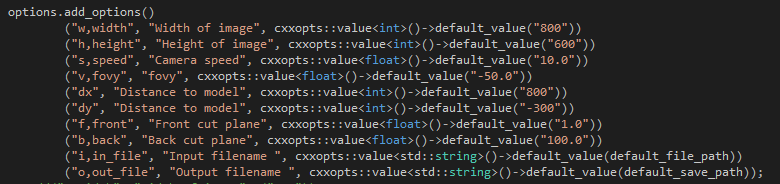
\includegraphics[width=1\linewidth]{images/TriangleDrawer/1/option.png}}
\caption{Параметры}
\label{ris:image}
\end{figure}

Результат работы: 

\begin{figure}[h!]
\begin{minipage}[h]{0.47\linewidth}
\center{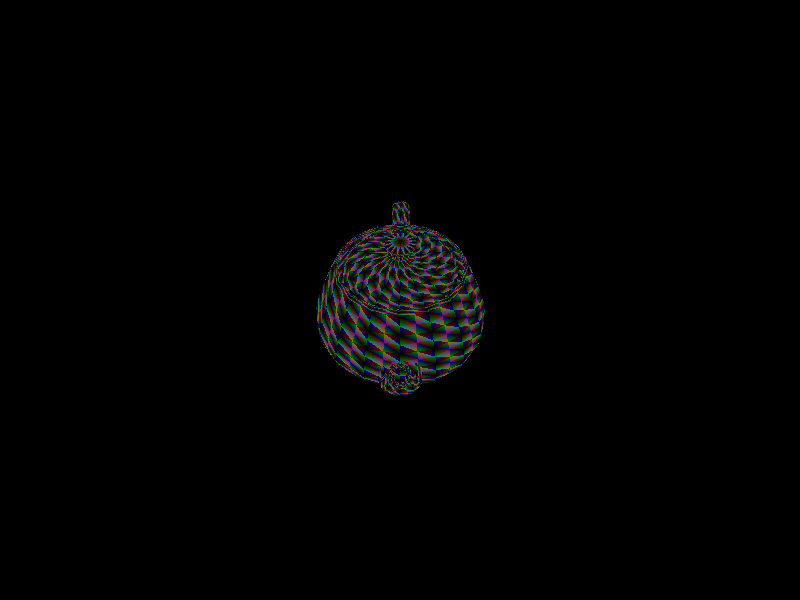
\includegraphics[width=1\linewidth]{images/TriangleDrawer/1/teapot0.png}} a) \\
\end{minipage}
\hfill
\begin{minipage}[h]{0.47\linewidth}
\center{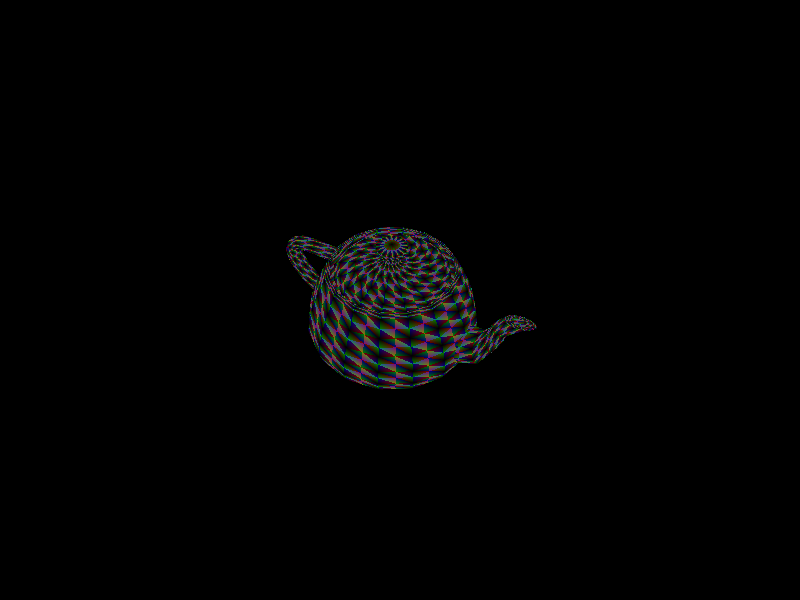
\includegraphics[width=1\linewidth]{images/TriangleDrawer/1/teapot1.png}} \\b)
\end{minipage}
\vfill
\begin{minipage}[h]{0.47\linewidth}
\center{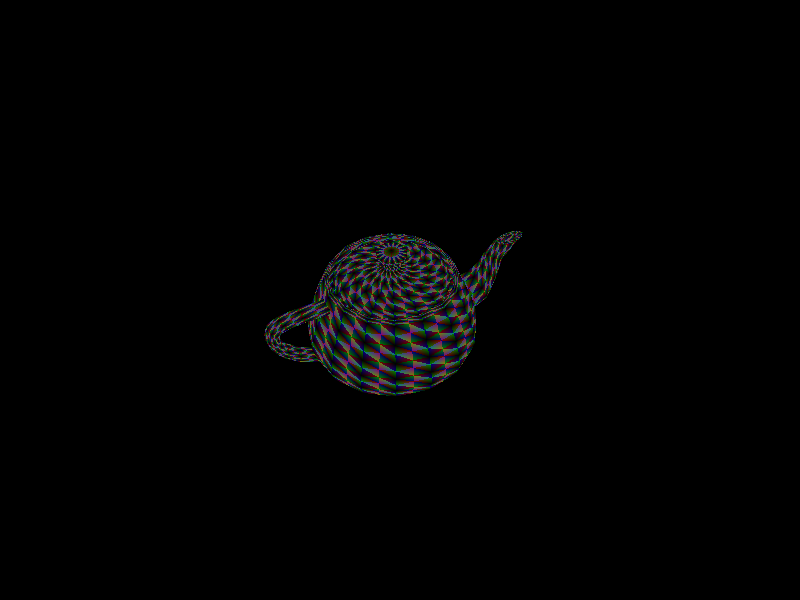
\includegraphics[width=1\linewidth]{images/TriangleDrawer/1/teapot2.png}} c) \\
\end{minipage}
\hfill
\begin{minipage}[h]{0.47\linewidth}
\center{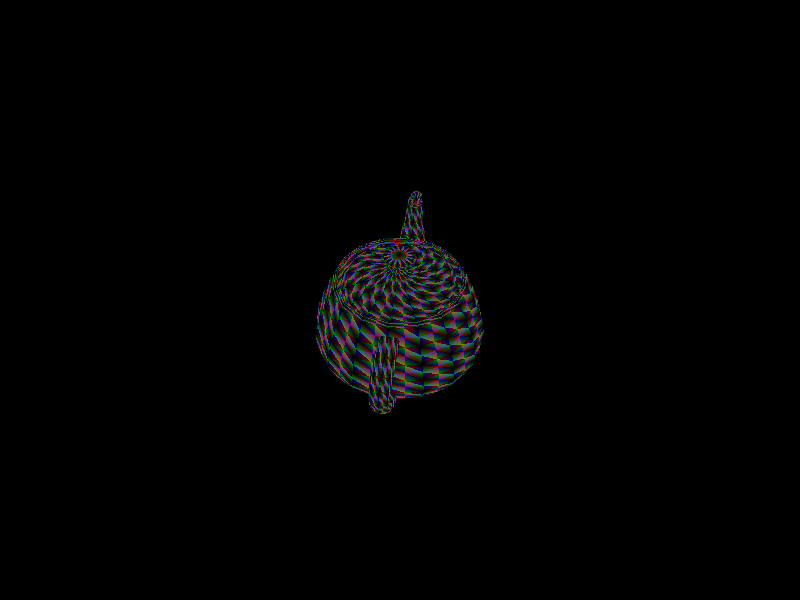
\includegraphics[width=1\linewidth]{images/TriangleDrawer/1/teapot3.png}} d) \\
\end{minipage}
\caption{Последовательно создаваемые изображения}
\label{ris:experimentalcorrelationsignals}
\end{figure}

Приведем еще несколько результатов, изменяя параметры камеры:

\clearpage
Параметры:

\begin{figure}[h!]
\center{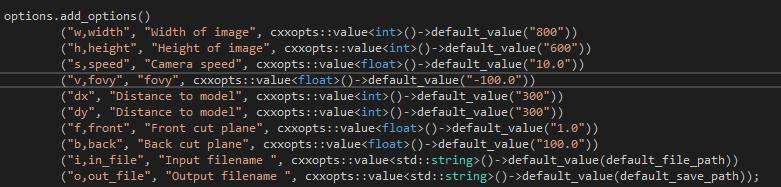
\includegraphics[width=1\linewidth]{images/TriangleDrawer/2/options.png}}
\caption{Параметры}
\label{ris:image}
\end{figure}

Результат работы: 

\begin{figure}[h!]
\begin{minipage}[h]{0.47\linewidth}
\center{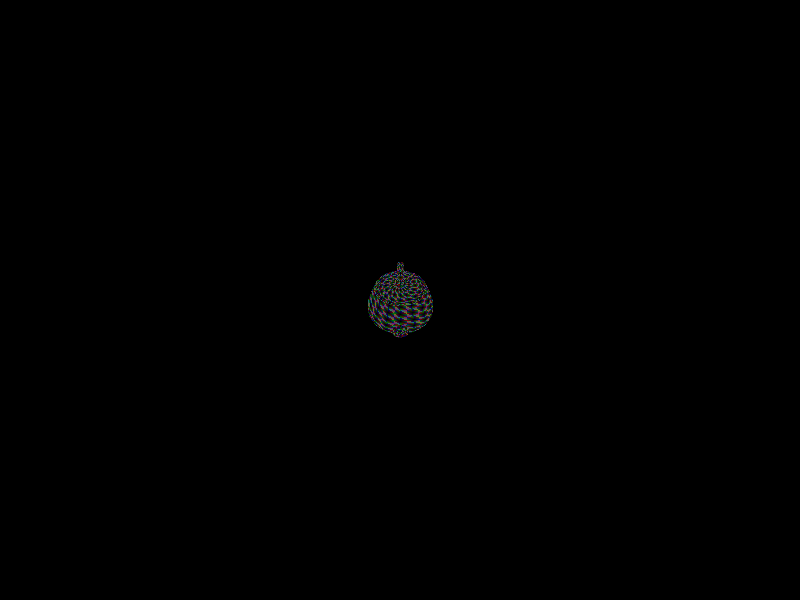
\includegraphics[width=1\linewidth]{images/TriangleDrawer/2/teapot0.png}} a) \\
\end{minipage}
\hfill
\begin{minipage}[h]{0.47\linewidth}
\center{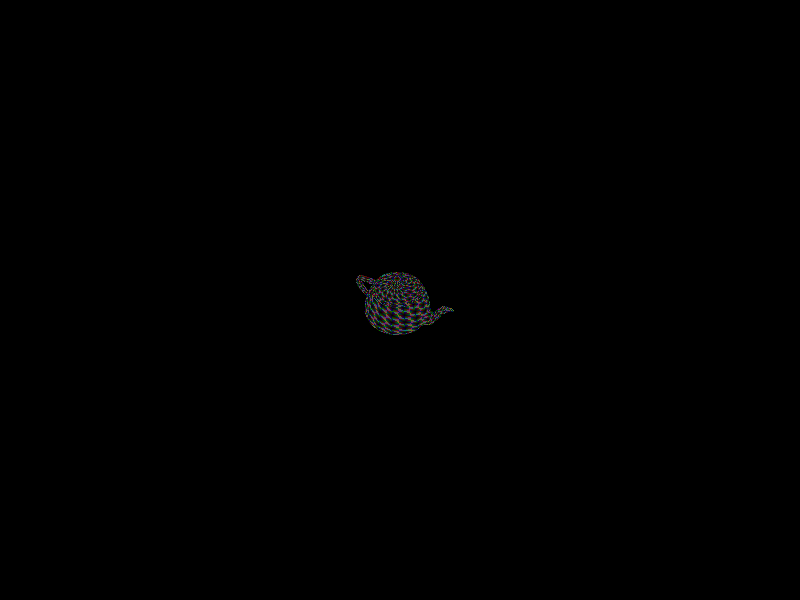
\includegraphics[width=1\linewidth]{images/TriangleDrawer/2/teapot1.png}} \\b)
\end{minipage}
\vfill
\begin{minipage}[h]{0.47\linewidth}
\center{
\includegraphics[width=1\linewidth]{images/TriangleDrawer/2/teapot2.png}} c) \\
\end{minipage}
\hfill
\begin{minipage}[h]{0.47\linewidth}
\center{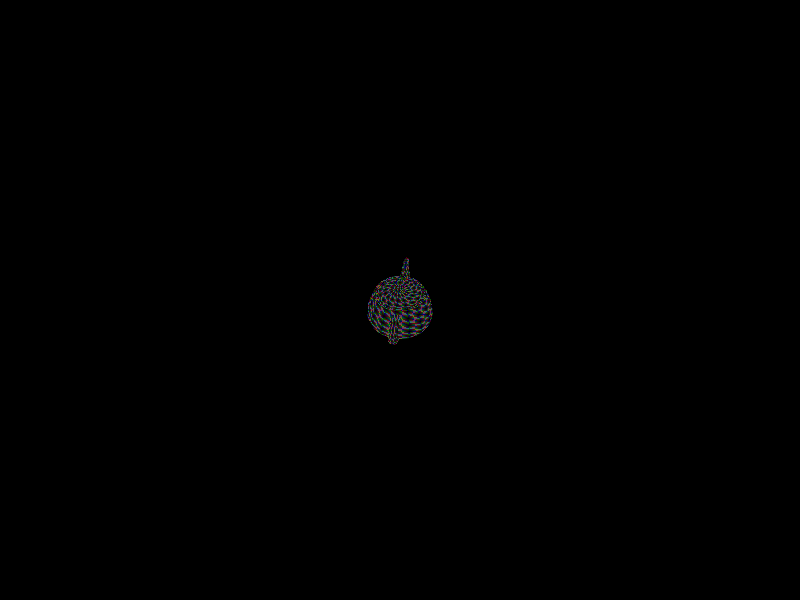
\includegraphics[width=1\linewidth]{images/TriangleDrawer/2/teapot3.png}} d) \\
\end{minipage}
\caption{Последовательно создаваемые изображения}
\label{ris:experimentalcorrelationsignals}
\end{figure}



\clearpage
Параметры:

\begin{figure}[h!]
\center{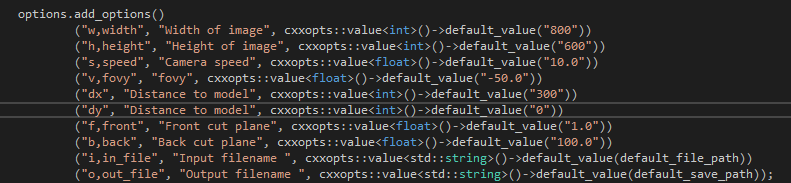
\includegraphics[width=1\linewidth]{images/TriangleDrawer/5/options.png}}
\caption{Параметры}
\label{ris:image}
\end{figure}

Результат работы: 

\begin{figure}[h!]
\begin{minipage}[h]{0.47\linewidth}
\center{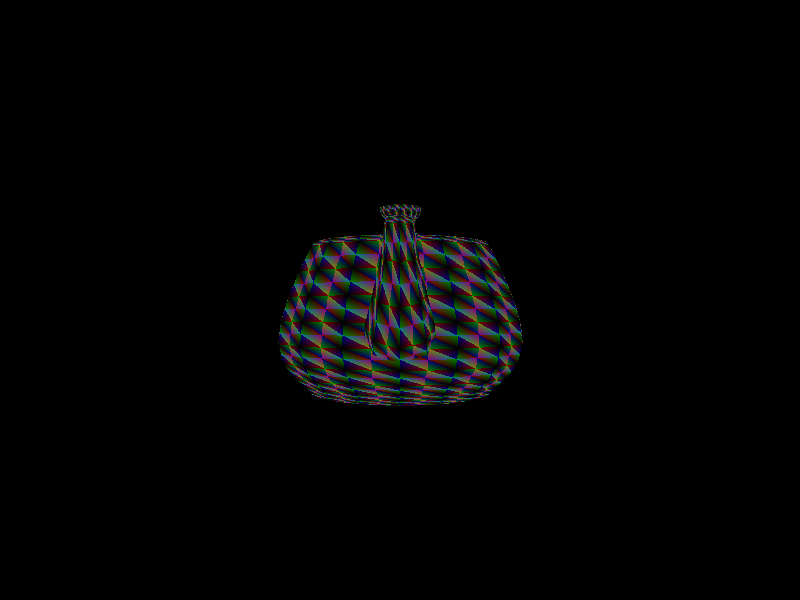
\includegraphics[width=1\linewidth]{images/TriangleDrawer/5/teapot0.png}} a) \\
\end{minipage}
\hfill
\begin{minipage}[h]{0.47\linewidth}
\center{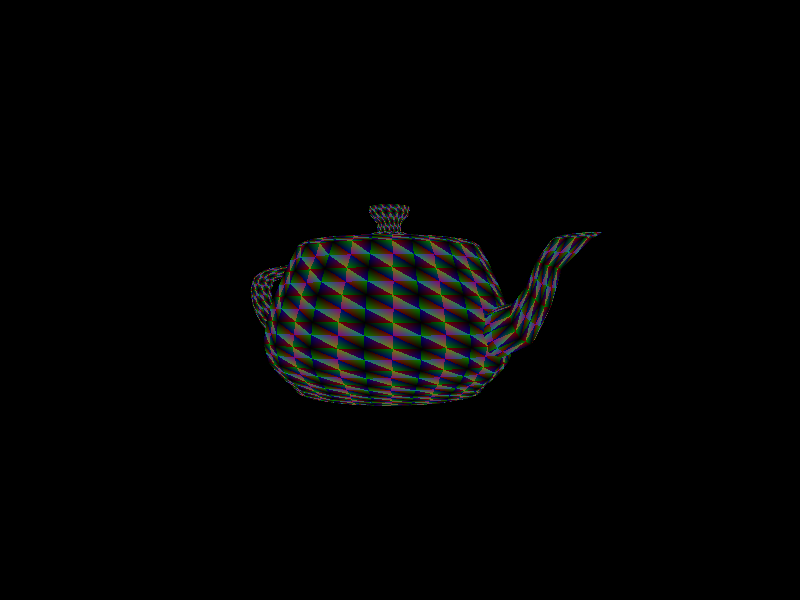
\includegraphics[width=1\linewidth]{images/TriangleDrawer/5/teapot1.png}} \\b)
\end{minipage}
\vfill
\begin{minipage}[h]{0.47\linewidth}
\center{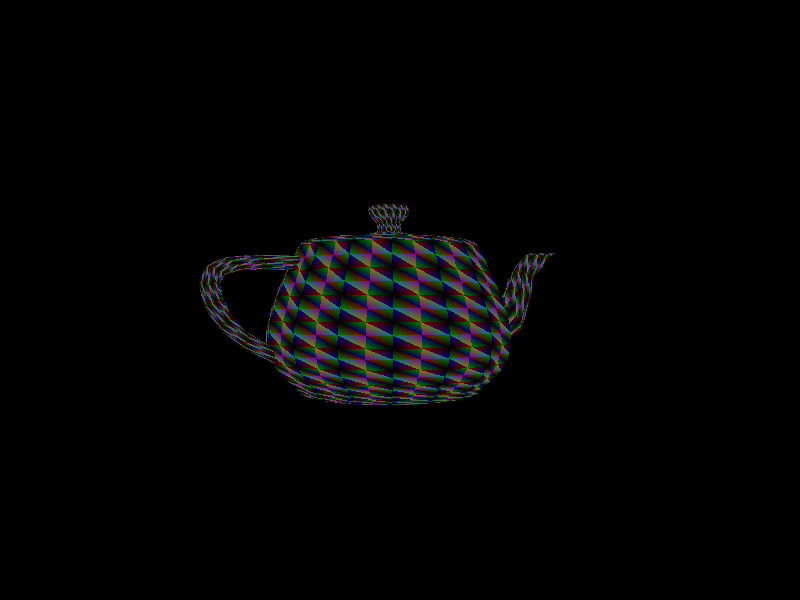
\includegraphics[width=1\linewidth]{images/TriangleDrawer/5/teapot2.png}} c) \\
\end{minipage}
\hfill
\begin{minipage}[h]{0.47\linewidth}
\center{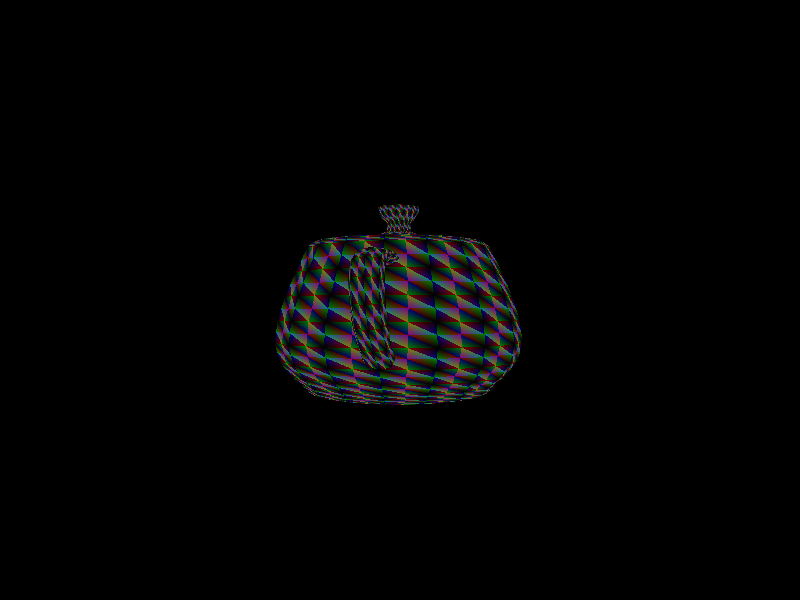
\includegraphics[width=1\linewidth]{images/TriangleDrawer/5/teapot3.png}} d) \\
\end{minipage}
\caption{Последовательно создаваемые изображения}
\label{ris:experimentalcorrelationsignals}
\end{figure}


\clearpage
Параметры:

\begin{figure}[h!]
\center{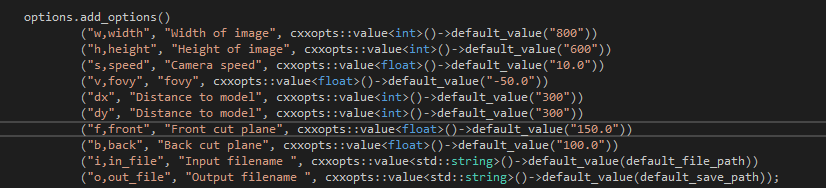
\includegraphics[width=1\linewidth]{images/TriangleDrawer/6/options.png}}
\caption{Параметры}
\label{ris:image}
\end{figure}

Результат работы: 

\begin{figure}[h!]
\begin{minipage}[h]{0.47\linewidth}
\center{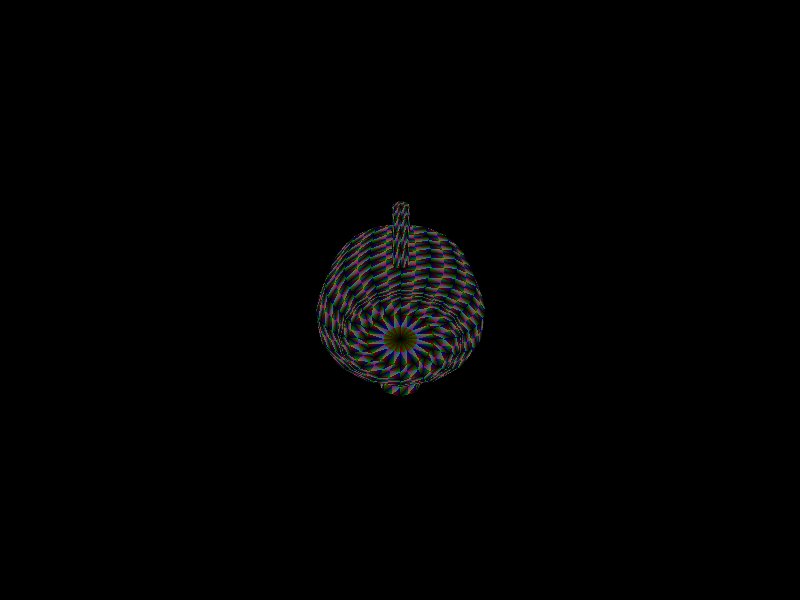
\includegraphics[width=1\linewidth]{images/TriangleDrawer/6/teapot0.png}} a) \\
\end{minipage}
\hfill
\begin{minipage}[h]{0.47\linewidth}
\center{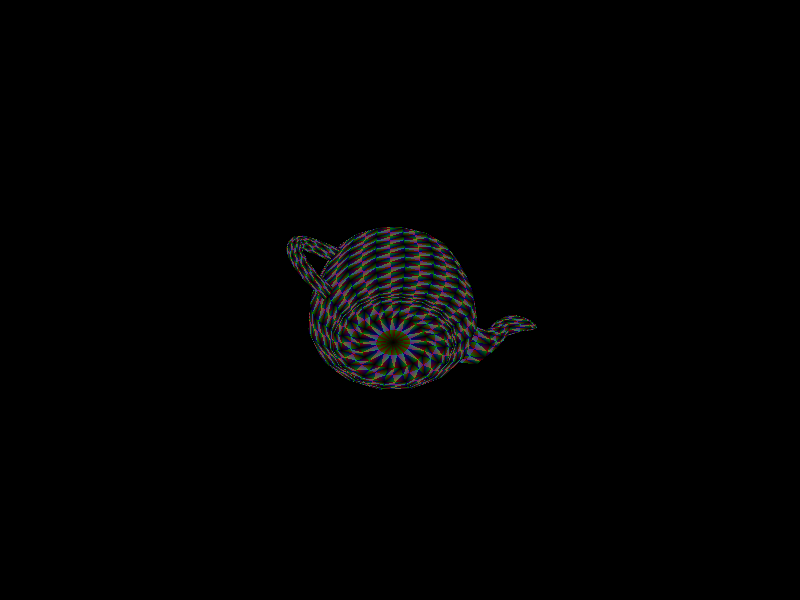
\includegraphics[width=1\linewidth]{images/TriangleDrawer/6/teapot1.png}} \\b)
\end{minipage}
\vfill
\begin{minipage}[h]{0.47\linewidth}
\center{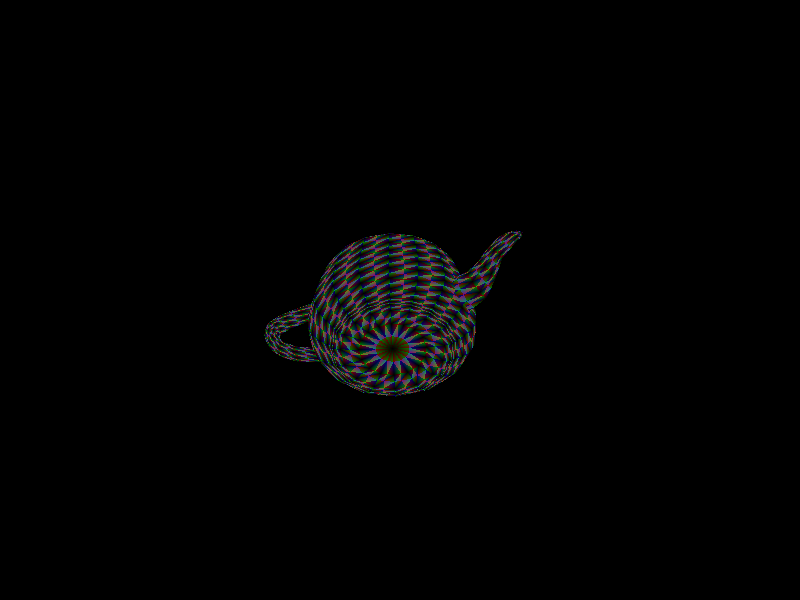
\includegraphics[width=1\linewidth]{images/TriangleDrawer/6/teapot2.png}} c) \\
\end{minipage}
\hfill
\begin{minipage}[h]{0.47\linewidth}
\center{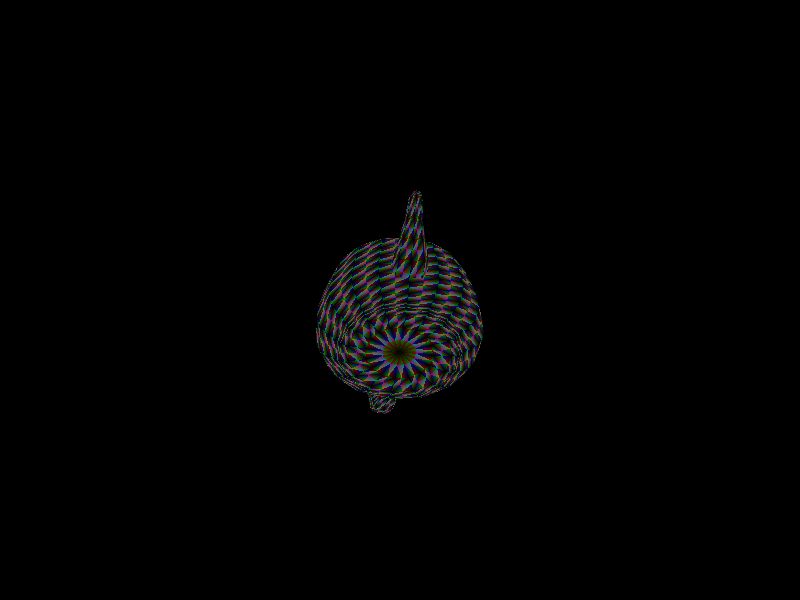
\includegraphics[width=1\linewidth]{images/TriangleDrawer/6/teapot3.png}} d) \\
\end{minipage}
\caption{Последовательно создаваемые изображения}
\label{ris:experimentalcorrelationsignals}
\end{figure}

\clearpage
\subsection{Z-буффер}



\begin{figure}[h!]
\begin{minipage}[h]{0.47\linewidth}
\center{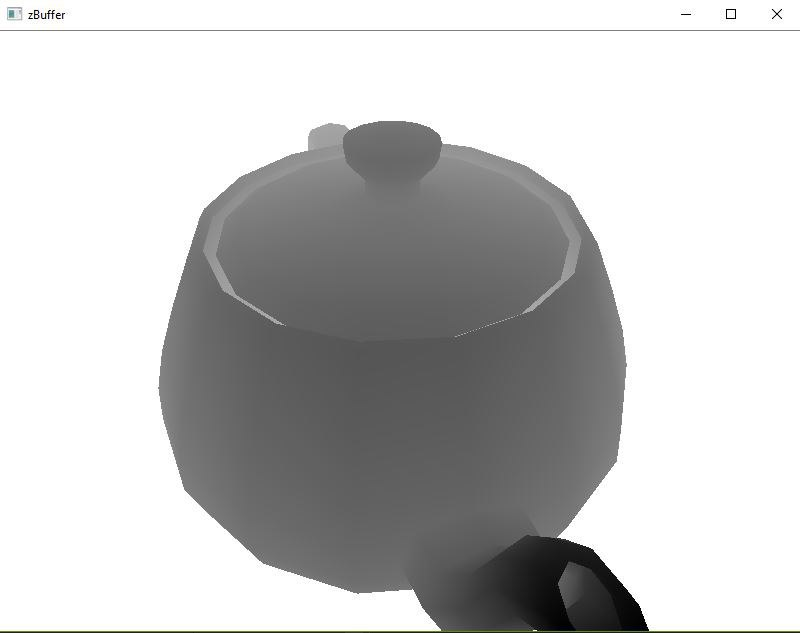
\includegraphics[width=1\linewidth]{images/zbuff/1.jpg}} a) \\
\end{minipage}
\hfill
\begin{minipage}[h]{0.47\linewidth}
\center{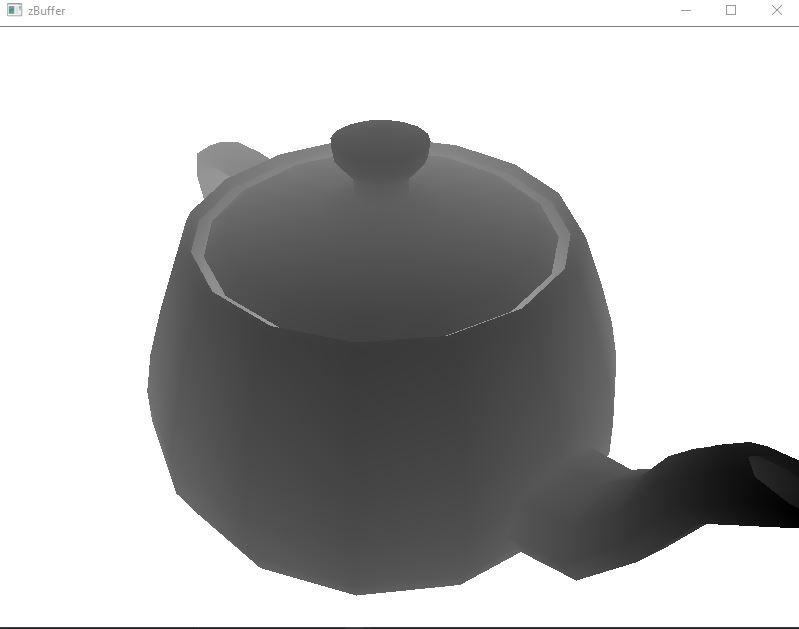
\includegraphics[width=1\linewidth]{images/zbuff/2.jpg}} \\b)
\end{minipage}
\vfill
\begin{minipage}[h]{0.47\linewidth}
\center{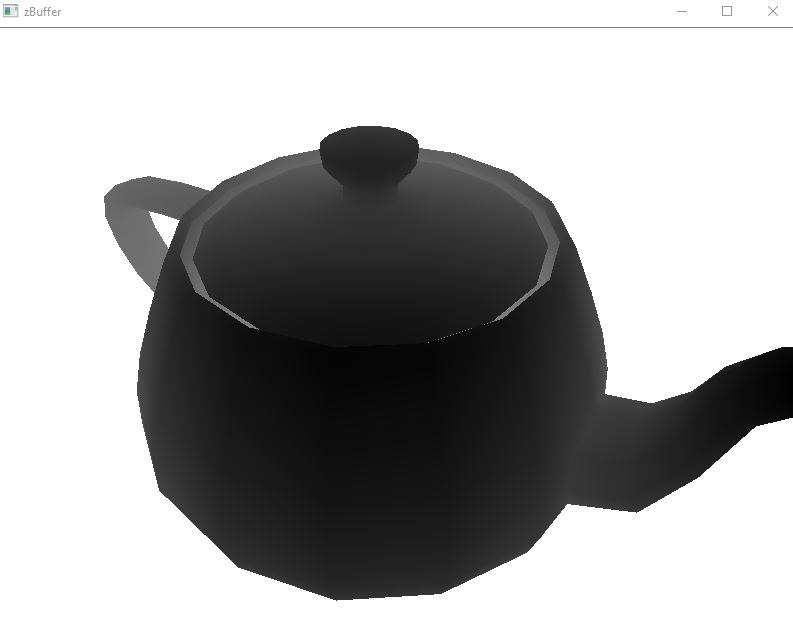
\includegraphics[width=1\linewidth]{images/zbuff/3.jpg}} c) \\
\end{minipage}
\hfill
\begin{minipage}[h]{0.47\linewidth}
\center{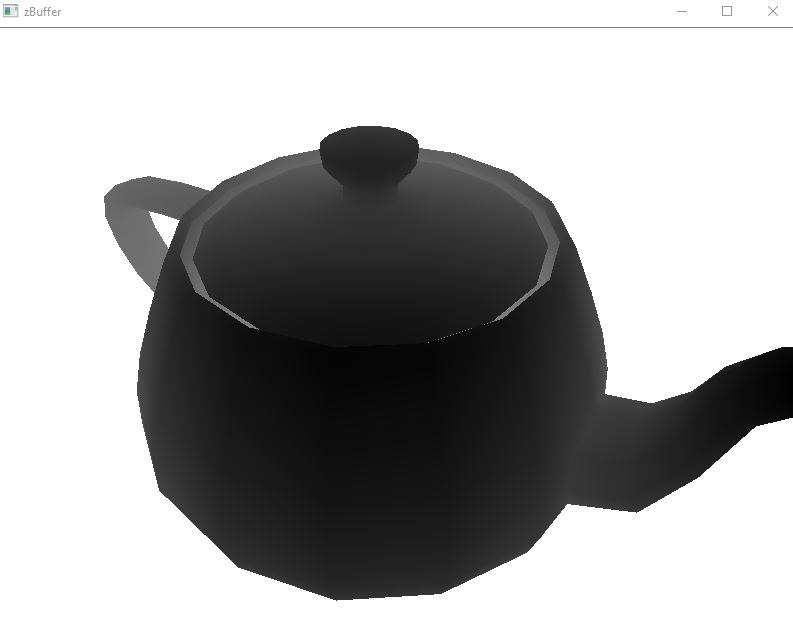
\includegraphics[width=1\linewidth]{images/zbuff/3.jpg}} d) \\
\end{minipage}
\caption{Последовательно создаваемые изображения}
\label{ris:experimentalcorrelationsignals}
\end{figure}



\clearpage
\section{Вывод}
В данной работе была изучена библиотека GLM и составлена программа для визуализации трехмерной модели в виде проволочного каркаса с использованием средств библиотеки OpenCV.

Результаты визуализации отвечают ожиданиям при заданном смещении, повороте и масштабе модели. Для создания более полного представления наблюдателя о внешнем виде исходной модели, необходимо в дальнейшем реализовать отображение поверхностей модели, посредством треугольников, учитывая, что используемая библиотека TinyObj позволяет проводить разбиение произвольного полигона на треугольники автоматически при чтении файла модели.

\clearpage
\section{Листинги}
\subsection{Листинг 1. main.cpp}
\lstinputlisting{listings/main.cpp}
\clearpage
\subsection{Листинг 2. Drawer.h}
\lstinputlisting{listings/Drawer.h}
\clearpage
\subsection{Листинг 3. render.h}
\lstinputlisting{listings/render.h}
\clearpage
\subsection{Листинг 4. transformers.h}
\lstinputlisting{listings/transformers.h}
\clearpage
\end{document}